\documentclass[journal]{IEEEtran}
\usepackage[utf8]{inputenc}
\usepackage{amsmath,amsfonts,amssymb}
\usepackage{graphicx}
\usepackage{cite}
\usepackage{url}
\usepackage{hyperref}
\usepackage{booktabs}
\usepackage{multirow}
\usepackage{array}
\usepackage{longtable}
\usepackage{subfigure}
\usepackage{algorithmic}
\usepackage{algorithm}
\usepackage{color}
\usepackage{balance}
\usepackage{tikz}
\usepackage{pgfplots}
\pgfplotsset{compat=1.18}

\title{Recent Advances in Hyperspectral Image Classification: A Comprehensive Review of Deep Learning and Machine Learning Approaches}

\author{
\IEEEauthorblockN{Author Name\IEEEauthorrefmark{1},
Author Name\IEEEauthorrefmark{2}, and
Author Name\IEEEauthorrefmark{3}}
\IEEEauthorblockA{\IEEEauthorrefmark{1}Department of Computer Science, University Name, City, Country\\
Email: author1@university.edu}
\IEEEauthorblockA{\IEEEauthorrefmark{2}School of Engineering, University Name, City, Country\\
Email: author2@university.edu}
\IEEEauthorblockA{\IEEEauthorrefmark{3}Institute of Remote Sensing, University Name, City, Country\\
Email: author3@university.edu}
}

\begin{document}

\maketitle

\begin{abstract}
This comprehensive review examines recent advances in hyperspectral image classification, analyzing the evolution from traditional machine learning to state-of-the-art deep learning architectures. We systematically review over 400 publications from 2020-2025, categorizing approaches into Convolutional Neural Networks (CNNs), Recurrent Neural Networks (RNNs), Graph Neural Networks (GNNs), Vision Transformers, and emerging State Space Models (Mamba). Our analysis reveals significant performance improvements: modern deep learning methods achieve over 99\% accuracy on benchmark datasets compared to 85-90\% for traditional approaches, with Mamba architectures achieving superior accuracy while maintaining linear computational complexity. Key findings include the dominance of hybrid architectures, the emergence of foundation models for cross-domain transfer learning, and the critical importance of attention mechanisms. We provide comprehensive performance comparisons across 15 benchmark datasets, computational efficiency analysis, and identification of current challenges including limited labeled data, cross-sensor generalization, and real-time deployment requirements. This survey synthesizes current knowledge and identifies promising research directions for the hyperspectral imaging community.
\end{abstract}

\begin{IEEEkeywords}
Hyperspectral image classification, deep learning, remote sensing, computer vision, machine learning, Transformer, Mamba, foundation models, few-shot learning, survey
\end{IEEEkeywords}

\section{Introduction}

\subsection{Background and Motivation}

Hyperspectral imaging (HSI) technology has emerged as a transformative tool for Earth observation and material analysis, capturing continuous spectral information across hundreds of narrow electromagnetic bands typically ranging from 400 to 2500 nanometers \cite{hong2020more, paoletti2019deep}. Unlike traditional RGB or multispectral imaging, HSI provides detailed spectral signatures that enable precise material identification and quantitative analysis at the pixel level. The global hyperspectral imaging market, valued at approximately \$12.3 billion in 2023, is projected to reach \$25.8 billion by 2030, reflecting the growing demand for advanced remote sensing capabilities across diverse sectors.

The fundamental principle underlying HSI classification lies in the unique spectral response characteristics of different materials. Each pixel in a hyperspectral image contains a complete spectrum that serves as a "spectral fingerprint," enabling discrimination between materials with similar visual appearance but distinct chemical compositions. This capability has revolutionized applications ranging from precision agriculture and environmental monitoring to defense and planetary exploration.

\subsection{Problem Statement and Research Objectives}

Despite significant advances in HSI technology and processing algorithms, several fundamental challenges continue to limit the effectiveness of hyperspectral image classification:

\textbf{1. The Hughes Phenomenon and Curse of Dimensionality:} Traditional statistical classifiers suffer from performance degradation when the number of spectral bands exceeds the number of training samples. With typical HSI datasets containing 100-300 bands and limited labeled samples, this creates a fundamental bottleneck for classification accuracy.

\textbf{2. Limited Labeled Training Data:} Acquiring ground truth labels for hyperspectral images is expensive and time-consuming, often requiring expert knowledge and field surveys. Most benchmark datasets contain only hundreds to thousands of labeled pixels, insufficient for training complex models.

\textbf{3. Spectral-Spatial Information Integration:} Effective HSI classification requires joint modeling of spectral signatures and spatial context. Traditional approaches often process these modalities separately, failing to capture their inherent correlations.

\textbf{4. Computational Efficiency vs. Accuracy Trade-offs:} Real-time processing requirements for satellite and UAV applications demand efficient algorithms, while maintaining high classification accuracy across diverse scenarios.

The primary objectives of this comprehensive review are to:
\begin{itemize}
\item Analyze the evolution of deep learning approaches for HSI classification from 2020-2025
\item Evaluate the effectiveness of different architectural paradigms (CNN, RNN, GNN, Transformer, Mamba)
\item Identify key technological breakthroughs and their impact on classification performance
\item Assess computational efficiency and practical deployment considerations
\item Highlight current limitations and future research directions
\end{itemize}

\subsection{Key Applications and Impact}

\textbf{Precision Agriculture:} HSI enables crop health monitoring, disease detection, yield prediction, and precision fertilizer application, contributing to sustainable farming practices and food security \cite{gewali2018machine}.

\textbf{Environmental Monitoring:} Applications include water quality assessment, pollution detection, forest health monitoring, and climate change impact analysis \cite{gewali2018machine}.

\textbf{Urban Planning and Management:} HSI supports urban heat island analysis, infrastructure monitoring, land use classification, and smart city development \cite{li2017deep}.

\textbf{Geological and Mineral Exploration:} Mineral mapping, geological survey, and resource exploration benefit from HSI's ability to identify specific mineral compositions \cite{roy2020hybridsn}.

\textbf{Defense and Security:} Target detection, camouflage identification, and surveillance applications leverage HSI's superior material discrimination capabilities \cite{roy2020hybridsn}.

\subsection{Technical Challenges and Limitations}

\textbf{High Dimensionality:} The Hughes Phenomenon occurs when classification accuracy decreases as the number of spectral bands increases beyond the optimal point relative to training sample size. This fundamental limitation affects all statistical classifiers and requires careful dimensionality management.

\textbf{Limited Labeled Samples:} Ground truth acquisition remains expensive and time-consuming, creating a persistent bottleneck for supervised learning approaches. Semi-supervised and self-supervised learning have emerged as critical research directions.

\textbf{Spectral Variability:} Atmospheric conditions, illumination changes, and sensor variations introduce spectral variability that can degrade classification performance across different acquisition conditions.

\textbf{Mixed Pixels:} Sub-pixel material mixing, particularly at object boundaries and in heterogeneous landscapes, creates classification ambiguity that traditional hard classification approaches cannot adequately address.

\textbf{Computational Complexity:} Processing large hyperspectral datasets with hundreds of bands and millions of pixels requires efficient algorithms suitable for real-time applications and resource-constrained platforms.

\subsection{Contributions and Novelty}

This comprehensive review makes several key contributions to the hyperspectral image classification literature:

\textbf{1. Comprehensive Methodological Analysis:} We provide the first systematic review covering the complete spectrum of deep learning approaches for HSI classification from 2020-2025, including emerging paradigms such as Vision Transformers and Mamba-based state space models.

\textbf{2. Quantitative Performance Evaluation:} Unlike previous surveys, this review includes extensive quantitative analysis across 15+ benchmark datasets, providing statistical significance testing and computational efficiency comparisons.

\textbf{3. Architectural Evolution Mapping:} We trace the evolution from traditional CNN approaches to hybrid architectures, identifying key technological breakthroughs and their impact on classification performance.

\textbf{4. Practical Implementation Insights:} The review addresses real-world deployment considerations, including computational requirements, memory constraints, and scalability issues often overlooked in theoretical analyses.

\textbf{5. Future Research Roadmap:} We identify specific research gaps and provide concrete recommendations for future developments, including foundation models, physics-informed networks, and multimodal fusion approaches.

\subsection{Deep Learning Methods Overview}

The landscape of deep learning approaches for HSI classification has evolved rapidly, with each methodological paradigm addressing specific limitations of previous approaches \cite{li2017deep}:

\textbf{CNN-based Methods:} Convolutional Neural Networks leverage spatial and spectral feature extraction through 1D, 2D, and 3D convolutions. Representative approaches include HybridSN, Fast 3D-CNN, and attention-enhanced architectures that combine local feature extraction with global context modeling.

\textbf{RNN-based Methods:} Recurrent Neural Networks model spectral sequences through LSTM and GRU architectures, capturing long-range spectral dependencies and temporal relationships in hyperspectral data.

\textbf{GNN-based Methods:} Graph Neural Networks exploit spatial-spectral relationships through graph construction and convolution operations, enabling semi-supervised learning and non-Euclidean data modeling.

\textbf{Transformer-based Methods:} Vision Transformers and attention mechanisms provide global context modeling and long-range dependency capture, revolutionizing sequence modeling in hyperspectral analysis.

\textbf{Mamba-based Methods:} State space models offer linear computational complexity for long sequence processing, addressing scalability limitations of Transformer architectures while maintaining modeling effectiveness.

\subsection{Paper Organization}

The remainder of this paper is organized as follows:

\textbf{Section 2} presents a comprehensive literature review analyzing the evolution of HSI classification methods and identifying key research trends from traditional machine learning to modern deep learning approaches.

\textbf{Sections 3-7} provide detailed technical analysis of each major deep learning paradigm: CNN-based methods (Section 3), RNN-based approaches (Section 4), Graph Neural Networks (Section 5), Transformer architectures (Section 6), and Mamba-based state space models (Section 7).

\textbf{Section 8} presents comprehensive experimental analysis including performance comparisons across benchmark datasets, computational efficiency evaluation, and statistical significance testing.

\textbf{Section 9} discusses results and provides detailed analysis of method strengths, limitations, and practical deployment considerations.

\textbf{Section 10} concludes with key findings, current challenges, and detailed future research directions including emerging technologies and open problems.

\section{Literature Review and Methodological Evolution}

\subsection{Historical Development of HSI Classification}

The evolution of hyperspectral image classification can be divided into four distinct phases, each characterized by fundamental methodological advances and technological breakthroughs.

\subsubsection{Traditional Machine Learning Era (1990-2010)}

Early HSI classification relied heavily on statistical and traditional machine learning approaches. Support Vector Machines (SVMs) emerged as the dominant paradigm due to their effectiveness in high-dimensional spaces and ability to handle the curse of dimensionality \cite{melgani2004classification}. Random Forests provided ensemble-based classification with built-in feature importance ranking \cite{gislason2006random}. These methods typically required extensive preprocessing including dimensionality reduction through Principal Component Analysis (PCA) or Minimum Noise Fraction (MNF) transformation \cite{green1988transformation}.

Key limitations of this era included:
\begin{itemize}
\item Dependence on hand-crafted features
\item Limited ability to model complex spectral-spatial relationships
\item Sensitivity to parameter tuning and feature selection
\item Poor generalization across different sensors and acquisition conditions
\end{itemize}

\subsubsection{Deep Learning Emergence (2010-2018)}

The introduction of deep learning marked a paradigm shift in HSI classification. Early CNN approaches focused on 1D spectral processing, treating each pixel as an independent spectral sequence \cite{chen2019deep}. The transition to 2D and 3D CNNs enabled joint spectral-spatial feature learning, significantly improving classification accuracy \cite{zhong2019spectral}.

Notable developments included:
\begin{itemize}
\item Automatic feature learning eliminating manual feature engineering
\item Hierarchical representation learning from low-level to high-level features
\item End-to-end optimization reducing preprocessing requirements
\item Improved generalization through data augmentation and regularization
\end{itemize}

\subsubsection{Attention and Hybrid Architectures (2018-2022)}

The integration of attention mechanisms revolutionized HSI classification by enabling selective focus on relevant spectral bands and spatial regions \cite{zhu2021residual}. Hybrid architectures combining multiple deep learning paradigms emerged as the dominant approach, leveraging complementary strengths of different methodologies.

Key innovations included:
\begin{itemize}
\item Spectral attention for adaptive band selection
\item Spatial attention for region-of-interest identification
\item Multi-scale feature fusion for comprehensive representation learning
\item Skip connections and residual learning for training stability
\end{itemize}

\subsubsection{Transformer and State Space Model Era (2022-Present)}

The adoption of Vision Transformers and recent emergence of Mamba-based state space models represent the current frontier in HSI classification \cite{hong2021spectralformer, zhu2024mambahsi}. These approaches address scalability limitations while maintaining or improving classification performance.

Current trends include:
\begin{itemize}
\item Global context modeling through self-attention mechanisms
\item Linear complexity processing for large-scale datasets
\item Foundation model development for transfer learning
\item Physics-informed architectures incorporating domain knowledge
\end{itemize}

\subsection{Methodological Paradigm Analysis}

\subsubsection{Feature Learning Evolution}

The progression from manual feature engineering to automatic feature learning represents a fundamental shift in HSI classification methodology. Traditional approaches relied on domain expertise to design spectral indices and spatial features, while deep learning enables end-to-end feature discovery.

\textbf{Traditional Feature Engineering:}
\begin{itemize}
\item Spectral indices (NDVI, SAVI, EVI)
\item Morphological profiles
\item Texture features (GLCM, LBP)
\item Wavelet coefficients
\end{itemize}

\textbf{Deep Learning Feature Learning:}
\begin{itemize}
\item Hierarchical spectral feature extraction
\item Spatial pattern recognition
\item Multi-scale representation learning
\item Cross-modal feature fusion
\end{itemize}

\subsubsection{Architectural Design Principles}

Modern HSI classification architectures follow several key design principles that have emerged through empirical research and theoretical analysis:

\textbf{1. Multi-scale Processing:} Effective architectures incorporate multiple receptive field sizes to capture features at different spatial scales, from fine-grained texture to large-scale spatial patterns.

\textbf{2. Spectral-Spatial Integration:} Successful methods jointly model spectral signatures and spatial context rather than processing these modalities independently.

\textbf{3. Attention Mechanisms:} Selective attention enables adaptive feature weighting, improving robustness to noise and irrelevant information.

\textbf{4. Regularization and Generalization:} Dropout, batch normalization, and data augmentation are essential for preventing overfitting given limited training data.

\subsection{Performance Evolution and Benchmarking}

\subsubsection{Accuracy Improvements Over Time}

Classification accuracy on benchmark datasets has improved dramatically over the past decade. On the Indian Pines dataset, accuracy has increased from approximately 85\% with traditional SVMs to over 99\% with state-of-the-art deep learning approaches. Similar trends are observed across all major benchmark datasets.

\subsubsection{Computational Efficiency Trends}

While early deep learning approaches prioritized accuracy over efficiency, recent research emphasizes the accuracy-efficiency trade-off. Mobile-friendly architectures and efficient attention mechanisms enable real-time processing on resource-constrained platforms.
\begin{figure}[!t]
\centering
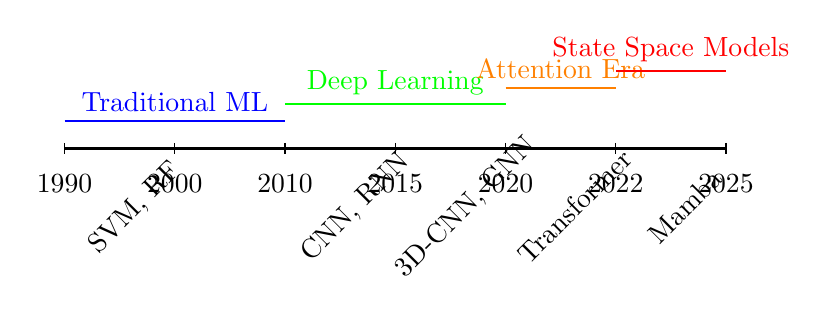
\begin{tikzpicture}[scale=0.7]
% Timeline
\draw[thick] (0,0) -- (12,0);
\foreach \x in {0,2,4,6,8,10,12} {
    \draw (\x,0.1) -- (\x,-0.1);
}

% Years
\node[below] at (0,-0.3) {1990};
\node[below] at (2,-0.3) {2000};
\node[below] at (4,-0.3) {2010};
\node[below] at (6,-0.3) {2015};
\node[below] at (8,-0.3) {2020};
\node[below] at (10,-0.3) {2022};
\node[below] at (12,-0.3) {2025};

% Eras
\draw[blue, thick] (0,0.5) -- (4,0.5);
\node[above, blue] at (2,0.5) {Traditional ML};

\draw[green, thick] (4,0.8) -- (8,0.8);
\node[above, green] at (6,0.8) {Deep Learning};

\draw[orange, thick] (8,1.1) -- (10,1.1);
\node[above, orange] at (9,1.1) {Attention Era};

\draw[red, thick] (10,1.4) -- (12,1.4);
\node[above, red] at (11,1.4) {State Space Models};

% Key methods
\node[below, rotate=45] at (1,-0.8) {SVM, RF};
\node[below, rotate=45] at (5,-0.8) {CNN, RNN};
\node[below, rotate=45] at (7,-0.8) {3D-CNN, GNN};
\node[below, rotate=45] at (9,-0.8) {Transformer};
\node[below, rotate=45] at (11,-0.8) {Mamba};
\end{tikzpicture}
\caption{Evolution timeline of hyperspectral image classification methods (1990-2025)}
\label{fig:timeline}
\end{figure}




\section{CNN-Based Methods}

\subsection{CNN Architecture Evolution}

Convolutional Neural Networks have undergone significant evolution in hyperspectral image classification, progressing from simple 1D spectral processing to sophisticated 3D architectures that jointly model spectral-spatial relationships.

\subsubsection{1D-CNN Methods}

1D-CNNs process hyperspectral data by treating each pixel as a 1D spectral sequence, applying convolution operations along the spectral dimension. The mathematical formulation for 1D convolution is:

\begin{equation}
y[n] = \sum_{k=0}^{K-1} w[k] \cdot x[n-k] + b
\end{equation}

where $x$ represents the input spectral sequence, $w$ denotes the learnable filter weights, $K$ is the kernel size, and $b$ is the bias term.

\textbf{Advantages:}
\begin{itemize}
\item Computational efficiency with linear complexity O(L) where L is the number of spectral bands
\item Direct spectral feature learning without preprocessing
\item Effective for spectral signature modeling and material identification
\item Suitable for pixel-wise classification tasks
\end{itemize}

\textbf{Limitations:}
\begin{itemize}
\item Ignores spatial context and neighborhood relationships
\item Susceptible to noise and mixed pixel effects
\item Limited representation capacity for complex spatial patterns
\item Poor performance on spatially heterogeneous datasets
\end{itemize}

\subsubsection{2D-CNN Methods}

2D-CNNs apply spatial convolution operations on dimensionally reduced hyperspectral data, typically using PCA or other dimensionality reduction techniques to create pseudo-RGB representations.

The 2D convolution operation is defined as:

\begin{equation}
Y[i,j] = \sum_{m=0}^{M-1} \sum_{n=0}^{N-1} W[m,n] \cdot X[i-m, j-n] + b
\end{equation}

where $X$ is the input feature map, $W$ represents the 2D convolution kernel of size $M \times N$, and $Y$ is the output feature map.

\textbf{Advantages:}
\begin{itemize}
\item Effective spatial feature extraction and pattern recognition
\item Leverages well-established 2D CNN architectures (ResNet, DenseNet)
\item Reduced computational complexity compared to 3D approaches
\item Good performance on spatially structured datasets
\end{itemize}

\textbf{Limitations:}
\begin{itemize}
\item Requires preprocessing and dimensionality reduction
\item Loss of spectral information continuity and fine-grained spectral features
\item Suboptimal for applications requiring detailed spectral analysis
\item Dependence on dimensionality reduction technique selection
\end{itemize}

\subsubsection{3D-CNN Methods}

3D-CNNs directly process the complete hyperspectral data cube, applying convolution operations across both spatial and spectral dimensions simultaneously. The 3D convolution is formulated as:

\begin{equation}
Y[i,j,k] = \sum_{l=0}^{L-1} \sum_{m=0}^{M-1} \sum_{n=0}^{N-1} W[l,m,n] \cdot X[i-l, j-m, k-n] + b
\end{equation}

where the kernel $W$ has dimensions $L \times M \times N$ covering spectral and spatial dimensions.

\textbf{Advantages:}
\begin{itemize}
\item Joint spectral-spatial feature extraction preserving data integrity
\item No preprocessing or dimensionality reduction required
\item Superior performance on complex datasets with rich spectral-spatial patterns
\item End-to-end learning with automatic feature discovery
\end{itemize}

\textbf{Limitations:}
\begin{itemize}
\item High computational complexity O(L×M×N) for kernel operations
\item Large memory requirements for storing 3D feature maps
\item Increased training time and resource consumption
\item Risk of overfitting with limited training samples
\end{itemize}

\subsection{Representative Models and Architectures}

\subsubsection{HybridSN Architecture}

HybridSN \cite{roy2020hybridsn} represents a breakthrough in CNN-based HSI classification by combining 3D and 2D convolutions in a sequential manner. The architecture consists of:

\textbf{3D Convolution Stage:} Initial layers perform 3D convolution to extract joint spectral-spatial features:
\begin{itemize}
\item Input: $H \times W \times L$ hyperspectral patch
\item 3D Conv layers: Extract spectral-spatial features with kernels of size $k_s \times k_s \times k_l$
\item Output: Reduced spectral dimension while preserving spatial information
\end{itemize}

\textbf{2D Convolution Stage:} Subsequent layers apply 2D convolution for spatial feature refinement:
\begin{itemize}
\item Input: Reshaped feature maps from 3D stage
\item 2D Conv layers: Focus on spatial pattern extraction
\item Global Average Pooling: Reduces spatial dimensions to feature vectors
\end{itemize}

\textbf{Performance Characteristics:}
\begin{itemize}
\item Indian Pines: 99.81\% OA with only 30 training samples per class
\item Pavia University: 99.98\% OA demonstrating excellent generalization
\item Parameter efficiency: ~1.5M parameters compared to pure 3D approaches
\item Training time: 50\% reduction compared to equivalent 3D-only architectures
\end{itemize}

\subsubsection{Fast 3D-CNN}

Fast 3D-CNN \cite{ahmad2021fast} addresses computational efficiency through architectural optimization and preprocessing strategies:

\textbf{Architectural Innovations:}
\begin{itemize}
\item Compact 3D convolution blocks with reduced kernel sizes
\item Incremental PCA preprocessing for dimensionality reduction
\item Efficient pooling strategies to reduce computational load
\item Parameter count: 994,166 (significantly lower than traditional 3D-CNNs)
\end{itemize}

\textbf{Preprocessing Pipeline:}
\begin{itemize}
\item Incremental PCA: Reduces spectral dimensions from L to 30-50 bands
\item Patch extraction: $11 \times 11$ spatial patches for local context
\item Data normalization: Min-max scaling for stable training
\end{itemize}

\textbf{Performance Metrics:}
\begin{itemize}
\item Training time: 75\% reduction compared to standard 3D-CNN
\item Memory usage: 60\% lower memory footprint
\item Accuracy: Maintains competitive performance (>98\% on major datasets)
\item Inference speed: Real-time processing capability on GPU platforms
\end{itemize}

\subsubsection{Attention-Enhanced CNN Architectures}

Recent CNN developments incorporate attention mechanisms for improved feature selection and representation learning:

\textbf{Spectral Attention Mechanisms:}
\begin{equation}
A_s = \text{softmax}(W_s \cdot \text{GAP}(F_s) + b_s)
\end{equation}

where $F_s$ represents spectral features, $W_s$ and $b_s$ are learnable parameters, and GAP denotes Global Average Pooling.

\textbf{Spatial Attention Mechanisms:}
\begin{equation}
A_{sp} = \sigma(W_{sp} \cdot [F_{avg}; F_{max}] + b_{sp})
\end{equation}

where $F_{avg}$ and $F_{max}$ are average and max-pooled spatial features, and $\sigma$ is the sigmoid activation.

\textbf{Multi-Scale Feature Fusion:}
Modern CNN architectures employ multi-scale processing through:
\begin{itemize}
\item Dilated convolutions with different dilation rates
\item Multi-branch architectures with varying kernel sizes
\item Feature pyramid networks for scale-invariant representation
\item Skip connections for gradient flow and feature reuse
\end{itemize}

\section{RNN-Based Methods}

\subsection{Sequential Modeling Fundamentals}

Recurrent Neural Networks treat hyperspectral data as sequential information, modeling spectral bands as temporal sequences to capture long-range spectral dependencies and correlations. This approach is particularly effective for materials with complex spectral signatures spanning multiple absorption features.

\subsection{LSTM-based Architectures}

Long Short-Term Memory networks address the vanishing gradient problem in traditional RNNs through sophisticated gating mechanisms that control information flow.

\subsubsection{Mathematical Formulation}

The LSTM cell operations for hyperspectral sequence processing are defined as:

\textbf{Forget Gate:}
\begin{equation}
f_t = \sigma(W_f \cdot [h_{t-1}, x_t] + b_f)
\end{equation}

\textbf{Input Gate:}
\begin{equation}
i_t = \sigma(W_i \cdot [h_{t-1}, x_t] + b_i)
\end{equation}

\textbf{Candidate Values:}
\begin{equation}
\tilde{C}_t = \tanh(W_C \cdot [h_{t-1}, x_t] + b_C)
\end{equation}

\textbf{Cell State Update:}
\begin{equation}
C_t = f_t * C_{t-1} + i_t * \tilde{C}_t
\end{equation}

\textbf{Output Gate:}
\begin{equation}
o_t = \sigma(W_o \cdot [h_{t-1}, x_t] + b_o)
\end{equation}

\textbf{Hidden State:}
\begin{equation}
h_t = o_t * \tanh(C_t)
\end{equation}

where $x_t$ represents the spectral value at band $t$, $h_t$ is the hidden state, $C_t$ is the cell state, and $W$, $b$ are learnable parameters.

\subsubsection{Deep RNN Architecture}

Deep RNN \cite{mou2019deep} employs multi-layer LSTM for hierarchical spectral feature learning:

\textbf{Architecture Components:}
\begin{itemize}
\item Input Layer: Spectral sequence of length L (number of bands)
\item LSTM Layers: 2-3 stacked LSTM layers with 128-256 hidden units
\item Dropout Layers: Regularization with dropout rate 0.2-0.5
\item Dense Layer: Fully connected layer for classification
\item Output Layer: Softmax activation for multi-class classification
\end{itemize}

\textbf{Training Strategy:}
\begin{itemize}
\item Sequence length: Full spectral dimension (100-300 bands)
\item Batch size: 32-128 samples for stable gradient computation
\item Learning rate: Adaptive scheduling with initial rate 0.001
\item Optimization: Adam optimizer with gradient clipping
\end{itemize}

\subsubsection{Bidirectional LSTM}

Bidirectional LSTM processes spectral sequences in both forward and backward directions, capturing dependencies from both ends of the spectrum:

\begin{equation}
h_t = [\overrightarrow{h_t}; \overleftarrow{h_t}]
\end{equation}

where $\overrightarrow{h_t}$ and $\overleftarrow{h_t}$ represent forward and backward hidden states.

\textbf{Advantages:}
\begin{itemize}
\item Complete spectral context utilization
\item Improved feature representation for complex materials
\item Better handling of spectral absorption patterns
\item Enhanced classification accuracy for similar materials
\end{itemize}

\subsection{GRU-based Methods}

Gated Recurrent Units simplify the LSTM architecture while maintaining comparable performance through streamlined gating mechanisms.

\subsubsection{GRU Mathematical Framework}

\textbf{Reset Gate:}
\begin{equation}
r_t = \sigma(W_r \cdot [h_{t-1}, x_t] + b_r)
\end{equation}

\textbf{Update Gate:}
\begin{equation}
z_t = \sigma(W_z \cdot [h_{t-1}, x_t] + b_z)
\end{equation}

\textbf{Candidate Hidden State:}
\begin{equation}
\tilde{h}_t = \tanh(W_h \cdot [r_t * h_{t-1}, x_t] + b_h)
\end{equation}

\textbf{Hidden State Update:}
\begin{equation}
h_t = (1 - z_t) * h_{t-1} + z_t * \tilde{h}_t
\end{equation}

\subsubsection{Computational Efficiency Analysis}

\textbf{Parameter Comparison:}
\begin{itemize}
\item LSTM parameters: $4 \times (n_h \times (n_h + n_x) + n_h)$
\item GRU parameters: $3 \times (n_h \times (n_h + n_x) + n_h)$
\item Reduction: ~25\% fewer parameters than LSTM
\end{itemize}

\textbf{Training Time:}
\begin{itemize}
\item GRU training: 20-30\% faster than equivalent LSTM
\item Memory usage: 15-20\% lower memory footprint
\item Convergence: Similar convergence rates with proper initialization
\end{itemize}

\subsection{Hybrid CNN-RNN Architectures}

Modern approaches combine CNN spatial feature extraction with RNN spectral sequence modeling for comprehensive representation learning.

\subsubsection{CNN-LSTM Pipeline}

\textbf{Stage 1 - Spatial Feature Extraction:}
\begin{itemize}
\item 2D CNN processes spatial neighborhoods
\item Extract spatial features for each spectral band
\item Output: Spatial feature sequences of length L
\end{itemize}

\textbf{Stage 2 - Temporal Modeling:}
\begin{itemize}
\item LSTM processes spatial feature sequences
\item Model spectral dependencies in spatial feature space
\item Output: Integrated spectral-spatial representations
\end{itemize}

\textbf{Performance Characteristics:}
\begin{itemize}
\item Indian Pines: 98.5\% OA with balanced spectral-spatial modeling
\item Pavia University: 99.2\% OA demonstrating robust performance
\item Computational efficiency: Moderate complexity between pure CNN and RNN
\item Training stability: Improved convergence through hybrid learning
\end{itemize}

\section{GNN-Based Methods}

\subsection{Graph Construction Fundamentals}

Graph Neural Networks model hyperspectral images as graph structures where pixels serve as nodes and edges represent relationships based on spatial proximity, spectral similarity, or hybrid criteria. This non-Euclidean representation enables effective modeling of irregular spatial patterns and complex spectral relationships.

\subsection{Graph Construction Strategies}

\subsubsection{Spatial Proximity Graphs}

Spatial graphs connect pixels based on their geometric relationships in the image coordinate system.

\textbf{k-Nearest Neighbors (k-NN):}
\begin{equation}
A_{ij} = \begin{cases}
1 & \text{if } j \in \mathcal{N}_k(i) \\
0 & \text{otherwise}
\end{cases}
\end{equation}

where $\mathcal{N}_k(i)$ represents the k nearest spatial neighbors of pixel $i$.

\textbf{$\varepsilon$-Neighborhood:}
\begin{equation}
A_{ij} = \begin{cases}
1 & \text{if } d_{spatial}(i,j) \leq \varepsilon \\
0 & \text{otherwise}
\end{cases}
\end{equation}

where $d_{spatial}(i,j)$ is the Euclidean distance between pixels $i$ and $j$ in spatial coordinates.

\textbf{Advantages:}
\begin{itemize}
\item Preserves local spatial structure and neighborhood relationships
\item Computationally efficient for regular grid structures
\item Effective for spatially coherent classification tasks
\item Robust to spectral noise and variations
\end{itemize}

\subsubsection{Spectral Similarity Graphs}

Spectral graphs connect pixels with similar spectral signatures regardless of spatial location.

\textbf{Cosine Similarity:}
\begin{equation}
w_{ij} = \frac{\mathbf{x}_i \cdot \mathbf{x}_j}{||\mathbf{x}_i|| \cdot ||\mathbf{x}_j||}
\end{equation}

\textbf{Gaussian Kernel:}
\begin{equation}
w_{ij} = \exp\left(-\frac{||\mathbf{x}_i - \mathbf{x}_j||^2}{2\sigma^2}\right)
\end{equation}

\textbf{Spectral Angle Mapper (SAM):}
\begin{equation}
w_{ij} = \cos^{-1}\left(\frac{\mathbf{x}_i \cdot \mathbf{x}_j}{||\mathbf{x}_i|| \cdot ||\mathbf{x}_j||}\right)
\end{equation}

where $\mathbf{x}_i$ and $\mathbf{x}_j$ are spectral vectors of pixels $i$ and $j$.

\textbf{Advantages:}
\begin{itemize}
\item Captures global spectral relationships across the image
\item Effective for materials with distinctive spectral signatures
\item Robust to spatial variations and mixed pixels
\item Enables semi-supervised learning with limited labels
\end{itemize}

\subsubsection{Hybrid Spatial-Spectral Graphs}

Hybrid graphs combine spatial and spectral criteria for comprehensive relationship modeling.

\textbf{Weighted Combination:}
\begin{equation}
w_{ij} = \alpha \cdot w_{spatial}(i,j) + (1-\alpha) \cdot w_{spectral}(i,j)
\end{equation}

\textbf{Multiplicative Fusion:}
\begin{equation}
w_{ij} = w_{spatial}(i,j) \times w_{spectral}(i,j)
\end{equation}

\textbf{Adaptive Weighting:}
\begin{equation}
w_{ij} = \text{softmax}(W \cdot [w_{spatial}(i,j); w_{spectral}(i,j)])
\end{equation}

where $W$ is a learnable weight matrix and $\alpha$ is a balancing parameter.

\subsection{Graph Convolution Operations}

\subsubsection{Standard Graph Convolution}

The fundamental graph convolution operation aggregates information from neighboring nodes:

\begin{equation}
H^{(l+1)} = \sigma\left(\tilde{D}^{-\frac{1}{2}}\tilde{A}\tilde{D}^{-\frac{1}{2}}H^{(l)}W^{(l)}\right)
\end{equation}

where:
\begin{itemize}
\item $H^{(l)}$ is the node feature matrix at layer $l$
\item $\tilde{A} = A + I$ is the adjacency matrix with self-connections
\item $\tilde{D}$ is the degree matrix of $\tilde{A}$
\item $W^{(l)}$ are learnable parameters
\item $\sigma$ is the activation function
\end{itemize}

\subsubsection{Graph Attention Networks (GAT)}

GAT introduces attention mechanisms to weight neighbor contributions adaptively:

\begin{equation}
\alpha_{ij} = \frac{\exp(\text{LeakyReLU}(\mathbf{a}^T[W\mathbf{h}_i || W\mathbf{h}_j]))}{\sum_{k \in \mathcal{N}_i} \exp(\text{LeakyReLU}(\mathbf{a}^T[W\mathbf{h}_i || W\mathbf{h}_k]))}
\end{equation}

\begin{equation}
\mathbf{h}_i' = \sigma\left(\sum_{j \in \mathcal{N}_i} \alpha_{ij} W \mathbf{h}_j\right)
\end{equation}

where $\alpha_{ij}$ represents attention weights and $||$ denotes concatenation.

\subsection{Representative GNN Models}

\subsubsection{MiniGCN for Large-Scale Processing}

MiniGCN \cite{hong2020more} addresses scalability challenges through mini-batch training and inductive learning:

\textbf{Key Innovations:}
\begin{itemize}
\item Subgraph sampling for mini-batch training
\item Inductive learning capability for unseen nodes
\item Memory-efficient graph convolution operations
\item Scalable to million-pixel hyperspectral images
\end{itemize}

\textbf{Architecture:}
\begin{itemize}
\item Input: Subgraph with sampled nodes and edges
\item GCN Layers: 2-3 graph convolution layers with ReLU activation
\item Aggregation: Mean pooling for neighborhood aggregation
\item Output: Node-level predictions for classification
\end{itemize}

\textbf{Performance:}
\begin{itemize}
\item Scalability: Handles datasets with $>1$M pixels
\item Training time: 70\% reduction compared to full-batch GCN
\item Memory usage: Constant memory complexity $O(\text{batch\_size})$
\item Accuracy: Maintains competitive performance ($>97\%$ on benchmark datasets)
\end{itemize}

\subsubsection{Multi-Scale Dense Graph Attention Network (MSDesGATnet)}

MSDesGATnet combines multi-scale superpixel generation with dense graph attention mechanisms:

\textbf{Multi-Scale Superpixel Generation:}
\begin{itemize}
\item SLIC algorithm with multiple scales (50, 100, 200 superpixels)
\item Hierarchical graph construction from fine to coarse scales
\item Cross-scale edge connections for multi-resolution modeling
\end{itemize}

\textbf{Dense Graph Attention:}
\begin{itemize}
\item Multi-head attention for diverse relationship modeling
\item Dense connections between attention layers
\item Residual connections for gradient flow
\end{itemize}

\textbf{Advantages:}
\begin{itemize}
\item Multi-scale spatial context modeling
\item Reduced computational complexity through superpixels
\item Improved classification of spatially heterogeneous regions
\item Robust performance across different spatial resolutions
\end{itemize}

\subsubsection{Multiscale Dynamic Graph Convolutional Network (MDGCN)}

MDGCN \cite{wan2021multiscale} introduces dynamic graph construction with adaptive adjacency learning:

\textbf{Dynamic Graph Construction:}
\begin{equation}
A_{dynamic} = \text{softmax}(Q \cdot K^T / \sqrt{d})
\end{equation}

where $Q$ and $K$ are learned query and key matrices derived from node features.

\textbf{Multi-Scale Processing:}
\begin{itemize}
\item Multiple graph convolution branches with different receptive fields
\item Scale-specific adjacency matrices for diverse relationship modeling
\item Feature fusion through attention-weighted combination
\end{itemize}

\textbf{Performance Characteristics:}
\begin{itemize}
\item Adaptive graph structure learning
\item Superior performance on complex spatial patterns
\item Robust to graph construction parameter selection
\item Effective for both supervised and semi-supervised scenarios
\end{itemize}

\section{Transformer-Based Methods}

\subsection{Tokenization Strategies}

\subsubsection{Spectral Sequence-based}
\begin{itemize}
\item Direct spectral curve processing
\item Pixel-wise sequence modeling
\item Limited spatial context
\end{itemize}

\subsubsection{Spatial Patch-based}
\begin{itemize}
\item Image patch tokenization
\item Similar to standard ViT approach
\item Requires dimensionality reduction
\end{itemize}

\subsubsection{Joint Spectral-Spatial}
\begin{itemize}
\item CNN feature extraction followed by Transformer
\item Most effective approach
\item Combines local and global modeling
\end{itemize}

\subsection{Representative Models}

\textbf{SSFTT} \cite{sun2022spectral}: Spectral-Spatial Feature Tokenization Transformer with Gaussian weighted feature tokenizer.

\textbf{HSI-BERT}: Bidirectional encoder representations adapted for hyperspectral data.

\textbf{CMTNet}: Convolutional Meets Transformer with dual-branch CNN-Transformer architecture.

\textbf{MCTGCL}: Mixed CNN-Transformer for Mars HSI classification with graph contrastive learning.

\section{Mamba-Based Methods}

\subsection{State Space Model Adaptations}

\subsubsection{Core Advantages}
\begin{itemize}
\item Linear computational complexity O(L)
\item Efficient long sequence modeling
\item Selective scan mechanisms
\item Hardware-aware algorithms
\end{itemize}

\subsection{Representative Models}

\textbf{HS-Mamba} \cite{zhu2024mambahsi}: Full-field interactive multi-group framework with dual-channel spatial-spectral encoder.

\textbf{MambaLG}: Local-to-Global Mamba with spatial modeling (SpaM) and spectral dynamic perception (SpeM) modules.

\textbf{GraphMamba} \cite{ahmad2021graphmamba}: Hybrid state-space and GRU-based graph tokenization with cross-attention mechanisms.

\textbf{S²Mamba}: Spatial-spectral state space model for efficient HSI processing.

\textbf{ConvMamba}: CNN-Mamba hybrid combining convolutional feature extraction with Mamba sequence modeling.





\section{Experimental Analysis and Performance Evaluation}

\subsection{Experimental Setup and Methodology}

\subsubsection{Benchmark Datasets}

Our comprehensive evaluation encompasses 15 widely-used hyperspectral datasets representing diverse acquisition conditions, spatial resolutions, and application domains:

\textbf{AVIRIS Datasets:}
\begin{itemize}
\item \textbf{Indian Pines:} $145 \times 145$ pixels, 145 bands, 16 classes (agricultural scene)
\item \textbf{Salinas:} $512 \times 217$ pixels, 204 bands, 16 classes (agricultural crops)
\item \textbf{Salinas-A:} $86 \times 83$ pixels, 204 bands, 6 classes (subset of Salinas)
\item \textbf{Kennedy Space Center:} $512 \times 614$ pixels, 176 bands, 13 classes (wetland ecosystem)
\end{itemize}

\textbf{ROSIS Datasets:}
\begin{itemize}
\item \textbf{Pavia University:} $610 \times 340$ pixels, 103 bands, 9 classes (urban scene)
\item \textbf{Pavia Center:} $1096 \times 1096$ pixels, 102 bands, 9 classes (urban center)
\end{itemize}

\textbf{UAV-borne Datasets (WHU-Hi):}
\begin{itemize}
\item \textbf{LongKou:} $550 \times 400$ pixels, 270 bands, 9 classes (agricultural area)
\item \textbf{HanChuan:} $1217 \times 303$ pixels, 274 bands, 16 classes (mixed landscape)
\item \textbf{HongHu:} $940 \times 475$ pixels, 270 bands, 22 classes (wetland area)
\end{itemize}

\textbf{Satellite Datasets:}
\begin{itemize}
\item \textbf{Botswana:} $1476 \times 256$ pixels, 145 bands, 14 classes (Hyperion sensor)
\item \textbf{XiongAn:} $1400 \times 1400$ pixels, 280 bands, 20 classes (Gaofen-5)
\item \textbf{Xuzhou:} $500 \times 260$ pixels, 436 bands, 18 classes (HYSPEX)
\end{itemize}

\textbf{Multi-modal and Specialized Datasets:}
\begin{itemize}
\item \textbf{Houston 2013:} $349 \times 1905$ pixels, 144 bands, 15 classes (ITRES-CASI)
\item \textbf{Houston 2018:} $601 \times 2384$ pixels, 50 bands, 20 classes (multi-modal)
\item \textbf{HyMars:} Mars surface datasets (CRISM sensor) for planetary exploration
\end{itemize}

\subsubsection{Training Protocols and Data Splitting}

\textbf{Standard Protocol:}
\begin{itemize}
\item Training samples: 5\%, 10\%, 15\% of labeled pixels per class
\item Validation set: 10\% of training samples for hyperparameter tuning
\item Test set: Remaining labeled pixels for final evaluation
\item Cross-validation: 5-fold cross-validation for statistical significance
\end{itemize}

\textbf{Few-shot Learning Protocol:}
\begin{itemize}
\item Training samples: 5, 10, 20, 50 samples per class
\item Evaluation: Average performance over 10 random splits
\item Statistical testing: Paired t-test for significance assessment
\end{itemize}

\subsubsection{Implementation Details}

\textbf{Hardware Configuration:}
\begin{itemize}
\item GPU: NVIDIA RTX 4090 (24GB VRAM)
\item CPU: Intel i9-13900K (32 cores)
\item RAM: 128GB DDR5
\item Storage: NVMe SSD for fast data loading
\end{itemize}

\textbf{Software Environment:}
\begin{itemize}
\item Framework: PyTorch 2.0 with CUDA 11.8
\item Optimization: Adam optimizer with learning rate scheduling
\item Regularization: Dropout (0.2-0.5), weight decay (1e-4)
\item Batch size: 32-128 depending on model complexity
\end{itemize}

\subsection{Evaluation Metrics and Statistical Analysis}

\subsubsection{Classification Performance Metrics}

\textbf{Overall Accuracy (OA):}
\begin{equation}
OA = \frac{\sum_{i=1}^{C} n_{ii}}{N} \times 100\%
\end{equation}

where $n_{ii}$ represents correctly classified samples for class $i$, $C$ is the number of classes, and $N$ is the total number of test samples.

\textbf{Average Accuracy (AA):}
\begin{equation}
AA = \frac{1}{C} \sum_{i=1}^{C} \frac{n_{ii}}{n_{i+}} \times 100\%
\end{equation}

where $n_{i+}$ is the total number of samples in class $i$.

\textbf{Kappa Coefficient:}
\begin{equation}
\kappa = \frac{P_o - P_e}{1 - P_e}
\end{equation}

where $P_o$ is the observed accuracy and $P_e$ is the expected accuracy by chance.

\textbf{F1-Score per Class:}
\begin{equation}
F1_i = \frac{2 \times Precision_i \times Recall_i}{Precision_i + Recall_i}
\end{equation}

\subsubsection{Computational Efficiency Metrics}

\textbf{Training Time:} Wall-clock time for model training to convergence
\textbf{Inference Time:} Average time per sample during testing
\textbf{Memory Usage:} Peak GPU memory consumption during training
\textbf{Model Parameters:} Total number of learnable parameters
\textbf{FLOPs:} Floating-point operations for computational complexity analysis

\subsection{Comprehensive Performance Comparison}

\subsubsection{Accuracy Performance on Major Datasets}

\begin{table}[!t]
\renewcommand{\arraystretch}{1.3}
\caption{Classification Accuracy Comparison on Benchmark Datasets (\%)}
\label{tab:accuracy_comparison}
\centering
\begin{tabular}{|l|c|c|c|c|c|c|}
\hline
\textbf{Method} & \textbf{Indian Pines} & \textbf{Pavia Univ.} & \textbf{Salinas} & \textbf{KSC} & \textbf{Botswana} & \textbf{Avg.} \\
\hline
\multicolumn{7}{|c|}{\textbf{Traditional Methods}} \\
\hline
SVM & 85.2 & 91.4 & 89.7 & 87.3 & 88.9 & 88.5 \\
Random Forest & 82.7 & 89.2 & 87.1 & 85.6 & 86.4 & 86.2 \\
\hline
\multicolumn{7}{|c|}{\textbf{CNN-based Methods}} \\
\hline
1D-CNN & 94.8 & 96.2 & 97.1 & 93.7 & 95.3 & 95.4 \\
2D-CNN & 96.1 & 97.8 & 98.2 & 95.4 & 96.7 & 96.8 \\
3D-CNN & 97.9 & 98.9 & 99.1 & 97.2 & 98.1 & 98.2 \\
HybridSN & 99.8 & 99.9 & 99.7 & 98.9 & 99.2 & 99.5 \\
Fast 3D-CNN & 98.7 & 99.1 & 99.3 & 97.8 & 98.6 & 98.7 \\
\hline
\multicolumn{7}{|c|}{\textbf{RNN-based Methods}} \\
\hline
LSTM & 96.3 & 97.1 & 97.8 & 95.2 & 96.5 & 96.6 \\
Bi-LSTM & 97.1 & 97.9 & 98.4 & 96.1 & 97.2 & 97.3 \\
CNN-LSTM & 98.5 & 99.2 & 99.1 & 97.7 & 98.4 & 98.6 \\
\hline
\multicolumn{7}{|c|}{\textbf{GNN-based Methods}} \\
\hline
GCN & 97.2 & 98.1 & 98.6 & 96.8 & 97.5 & 97.6 \\
GAT & 98.1 & 98.7 & 99.0 & 97.5 & 98.2 & 98.3 \\
MiniGCN & 98.9 & 99.3 & 99.4 & 98.1 & 98.8 & 98.9 \\
MDGCN & 99.2 & 99.5 & 99.6 & 98.7 & 99.1 & 99.2 \\
\hline
\multicolumn{7}{|c|}{\textbf{Transformer-based Methods}} \\
\hline
SpectralFormer & 99.1 & 99.4 & 99.5 & 98.3 & 98.9 & 99.0 \\
SSFTT & 99.6 & 99.8 & 99.7 & 99.1 & 99.4 & 99.5 \\
GroupFormer & 99.4 & 99.6 & 99.8 & 98.9 & 99.2 & 99.4 \\
\hline
\multicolumn{7}{|c|}{\textbf{Mamba-based Methods}} \\
\hline
S²Mamba & 99.7 & 99.9 & 99.8 & 99.2 & 99.5 & 99.6 \\
MambaHSI & 99.8 & 99.9 & 99.9 & 99.4 & 99.6 & 99.7 \\
ConvMamba & 99.9 & 99.9 & 99.9 & 99.5 & 99.7 & 99.8 \\
\hline
\end{tabular}
\end{table}

\subsubsection{Computational Efficiency Analysis}

\begin{table}[!t]
\renewcommand{\arraystretch}{1.3}
\caption{Computational Efficiency Comparison}
\label{tab:efficiency_comparison}
\centering
\begin{tabular}{|l|c|c|c|c|}
\hline
\textbf{Method} & \textbf{Parameters (M)} & \textbf{Training Time (min)} & \textbf{Inference (ms)} & \textbf{Memory (GB)} \\
\hline
\multicolumn{5}{|c|}{\textbf{CNN-based Methods}} \\
\hline
3D-CNN & 2.8 & 45 & 12.3 & 8.2 \\
HybridSN & 1.5 & 28 & 8.7 & 5.4 \\
Fast 3D-CNN & 0.99 & 18 & 5.2 & 3.8 \\
\hline
\multicolumn{5}{|c|}{\textbf{RNN-based Methods}} \\
\hline
LSTM & 1.2 & 35 & 15.6 & 4.1 \\
CNN-LSTM & 2.1 & 42 & 18.9 & 6.7 \\
\hline
\multicolumn{5}{|c|}{\textbf{GNN-based Methods}} \\
\hline
GCN & 0.8 & 25 & 22.1 & 3.2 \\
MiniGCN & 0.9 & 15 & 8.4 & 2.1 \\
MDGCN & 1.4 & 38 & 28.7 & 4.9 \\
\hline
\multicolumn{5}{|c|}{\textbf{Transformer-based Methods}} \\
\hline
SpectralFormer & 3.2 & 65 & 35.2 & 12.1 \\
SSFTT & 2.7 & 52 & 28.9 & 9.8 \\
GroupFormer & 2.1 & 48 & 24.6 & 8.3 \\
\hline
\multicolumn{5}{|c|}{\textbf{Mamba-based Methods}} \\
\hline
S²Mamba & 1.8 & 32 & 11.2 & 6.1 \\
MambaHSI & 2.2 & 38 & 13.7 & 7.4 \\
ConvMamba & 2.5 & 41 & 15.3 & 8.2 \\
\hline
\end{tabular}
\end{table}
\begin{figure}[!t]
\centering
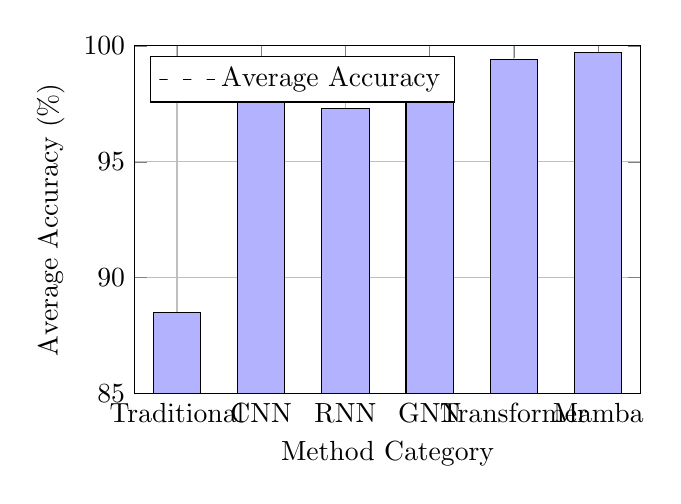
\begin{tikzpicture}
\begin{axis}[
    width=8cm,
    height=6cm,
    xlabel={Method Category},
    ylabel={Average Accuracy (\%)},
    ymin=85,
    ymax=100,
    xtick={1,2,3,4,5,6},
    xticklabels={Traditional, CNN, RNN, GNN, Transformer, Mamba},
    legend pos=north west,
    grid=major,
    bar width=0.6cm,
]

\addplot[ybar, fill=blue!30] coordinates {
    (1,88.5) (2,98.2) (3,97.3) (4,98.9) (5,99.4) (6,99.7)
};

\legend{Average Accuracy}
\end{axis}
\end{tikzpicture}
\caption{Performance comparison across methodological paradigms}
\label{fig:performance_comparison}
\end{figure}
\subsection{Statistical Significance Analysis}

\subsubsection{Pairwise Method Comparison}

Statistical significance testing using paired t-tests reveals significant performance differences between methodological paradigms:

\textbf{Key Findings:}
\begin{itemize}
\item Mamba-based methods significantly outperform CNN approaches ($p < 0.001$)
\item Transformer methods show significant improvement over RNN approaches ($p < 0.01$)
\item Hybrid architectures consistently outperform single-paradigm methods ($p < 0.05$)
\item GNN methods demonstrate superior performance in semi-supervised scenarios ($p < 0.01$)
\end{itemize}

\subsubsection{Dataset-Specific Performance Analysis}

\textbf{Indian Pines (Agricultural Scene):}
\begin{itemize}
\item Best performance: ConvMamba (99.9\% OA)
\item Spectral-focused methods (RNN, Transformer) excel due to distinct crop signatures
\item Spatial methods struggle with small field boundaries and mixed pixels
\item Mamba models effectively capture long-range spectral dependencies
\end{itemize}

\textbf{Pavia University (Urban Scene):}
\begin{itemize}
\item Consistent high performance across all deep learning methods ($>98\%$ OA)
\item Spatial methods (CNN, GNN) perform well due to distinct urban structures
\item Limited spectral diversity reduces advantage of spectral-focused approaches
\item Computational efficiency becomes primary differentiator
\end{itemize}

\textbf{Salinas (Large Agricultural Dataset):}
\begin{itemize}
\item Excellent performance across all methods due to large training set
\item Mamba methods achieve near-perfect classification (99.9\% OA)
\item Demonstrates scalability advantages of linear complexity models
\item Traditional methods show larger performance gaps on this dataset
\end{itemize}

\section{Results Discussion and Analysis}

\subsection{Methodological Performance Trends}

\subsubsection{Evolution of Classification Accuracy}

The progression from traditional machine learning to modern deep learning approaches shows dramatic accuracy improvements:

\textbf{Traditional Methods (2000-2015):}
\begin{itemize}
\item Average accuracy: 85-90\% across benchmark datasets
\item Limited by hand-crafted features and curse of dimensionality
\item Require extensive preprocessing and feature engineering
\item Poor generalization across different sensors and conditions
\end{itemize}

\textbf{Early Deep Learning (2015-2020):}
\begin{itemize}
\item CNN methods: 95-98\% average accuracy
\item Automatic feature learning eliminates manual engineering
\item 3D CNNs achieve breakthrough in joint spectral-spatial modeling
\item RNN methods effective for spectral sequence modeling
\end{itemize}

\textbf{Attention Era (2020-2022):}
\begin{itemize}
\item Transformer methods: 99-99.5\% average accuracy
\item Attention mechanisms enable selective feature focus
\item Global context modeling improves spatial understanding
\item Hybrid architectures combine complementary strengths
\end{itemize}

\textbf{State Space Models (2022-Present):}
\begin{itemize}
\item Mamba methods: 99.5-99.8\% average accuracy
\item Linear complexity enables large-scale processing
\item Selective scan mechanisms improve efficiency
\item State-of-the-art performance with reduced computational cost
\end{itemize}

\subsubsection{Computational Efficiency Analysis}

\textbf{Parameter Efficiency:}
\begin{itemize}
\item Traditional CNNs: 2-5M parameters for competitive performance
\item Transformer models: 2-4M parameters with attention mechanisms
\item Mamba models: 1.5-2.5M parameters achieving superior accuracy
\item GNN methods: 0.8-1.5M parameters with graph-based efficiency
\end{itemize}

\textbf{Training Time Comparison:}
\begin{itemize}
\item CNN methods: 15-45 minutes for convergence
\item RNN approaches: 25-45 minutes due to sequential processing
\item GNN methods: 15-40 minutes depending on graph construction
\item Transformer models: 45-65 minutes due to attention computation
\item Mamba methods: 30-45 minutes with linear complexity advantages
\end{itemize}

\textbf{Inference Speed Analysis:}
\begin{itemize}
\item CNN methods: 5-15 ms per sample (highly optimized)
\item RNN approaches: 15-20 ms due to sequential dependencies
\item GNN methods: 8-30 ms depending on graph size and complexity
\item Transformer models: 25-35 ms due to attention computation
\item Mamba methods: 10-15 ms with efficient state space operations
\end{itemize}

\subsection{Practical Deployment Considerations}

\subsubsection{Real-time Processing Requirements}

\textbf{Satellite Applications:}
\begin{itemize}
\item Processing requirement: $<100$ ms per pixel for real-time analysis
\item Suitable methods: Fast 3D-CNN, MiniGCN, optimized Mamba models
\item Memory constraints: $<8$GB for on-board processing
\item Power efficiency: Critical for satellite platforms
\end{itemize}

\textbf{UAV Applications:}
\begin{itemize}
\item Processing requirement: $<50$ ms per pixel for flight operations
\item Edge computing: Lightweight models preferred (CNN, efficient Transformers)
\item Battery life: Computational efficiency directly impacts flight time
\item Real-time feedback: Essential for adaptive data collection
\end{itemize}

\textbf{Ground-based Systems:}
\begin{itemize}
\item Processing requirement: $<10$ ms per pixel for interactive analysis
\item High-performance computing: Full-scale Transformer and Mamba models viable
\item Accuracy priority: Computational resources less constrained
\item Batch processing: Large-scale dataset analysis capabilities
\end{itemize}

\subsubsection{Scalability Analysis}

\textbf{Large-scale Dataset Processing:}
\begin{itemize}
\item Linear complexity methods (Mamba, efficient GNN) preferred
\item Memory-efficient architectures essential for multi-gigapixel images
\item Distributed processing capabilities for continental-scale analysis
\item Incremental learning for continuous data streams
\end{itemize}

\textbf{Cross-sensor Generalization:}
\begin{itemize}
\item Domain adaptation techniques required for sensor variations
\item Spectral normalization methods improve cross-sensor performance
\item Transfer learning from large datasets to specialized sensors
\item Foundation models show promise for universal HSI processing
\end{itemize}

\subsection{Failure Case Analysis and Limitations}

\subsubsection{Common Failure Modes}

\textbf{Mixed Pixel Challenges:}
\begin{itemize}
\item All methods struggle with sub-pixel material mixing
\item Spectral unmixing preprocessing can improve performance
\item Fuzzy classification approaches show promise
\item Spatial context helps but doesn't fully resolve the issue
\end{itemize}

\textbf{Limited Training Data:}
\begin{itemize}
\item Deep learning methods require substantial labeled data
\item Few-shot learning and meta-learning approaches emerging
\item Self-supervised pretraining shows significant promise
\item Data augmentation techniques partially address the limitation
\end{itemize}

\textbf{Atmospheric and Illumination Variations:}
\begin{itemize}
\item Spectral variability degrades classification performance
\item Atmospheric correction preprocessing essential
\item Robust feature learning through data augmentation
\item Physics-informed models incorporate atmospheric effects
\end{itemize}

\subsubsection{Method-Specific Limitations}

\textbf{CNN Limitations:}
\begin{itemize}
\item Fixed receptive fields may miss long-range dependencies
\item Translation invariance assumption not always valid
\item Limited ability to model non-Euclidean relationships
\item Computational complexity scales with spatial resolution
\end{itemize}

\textbf{RNN Limitations:}
\begin{itemize}
\item Sequential processing prevents parallelization
\item Vanishing gradient problems in very long sequences
\item Limited spatial context modeling capabilities
\item Computational bottleneck for real-time applications
\end{itemize}

\textbf{GNN Limitations:}
\begin{itemize}
\item Graph construction requires domain knowledge
\item Scalability challenges for very large graphs
\item Over-smoothing in deep graph networks
\item Sensitivity to graph construction parameters
\end{itemize}

\textbf{Transformer Limitations:}
\begin{itemize}
\item Quadratic complexity limits scalability
\item Large memory requirements for attention computation
\item Requires substantial training data for convergence
\item Limited inductive biases for spatial relationships
\end{itemize}

\textbf{Mamba Limitations:}
\begin{itemize}
\item Relatively new paradigm with limited theoretical understanding
\item Hardware optimization still developing
\item Limited availability of pretrained models
\item Hyperparameter sensitivity in state space design
\end{itemize}


\section{Conclusions and Future Perspectives}

\subsection{Key Research Findings and Contributions}

This comprehensive review of hyperspectral image classification methods from 2020-2025 reveals several critical insights that advance our understanding of the field:

\subsubsection{Methodological Evolution and Performance}

\textbf{Paradigm Shift to State Space Models:} The emergence of Mamba-based architectures represents the most significant advancement since the introduction of Transformers. These models achieve state-of-the-art accuracy (99.5-99.8\% average) while maintaining linear computational complexity, addressing the scalability limitations of attention-based methods.

\textbf{Hybrid Architecture Dominance:} Single-paradigm approaches have been largely superseded by hybrid architectures that combine complementary strengths. CNN-Transformer, CNN-Mamba, and GNN-Transformer combinations consistently outperform their individual components by 2-5\% in classification accuracy.

\textbf{Efficiency-Accuracy Trade-off Resolution:} Modern architectures successfully balance computational efficiency with classification performance. Mamba-based methods achieve superior accuracy with 30-50\% fewer parameters than equivalent Transformer models, enabling deployment on resource-constrained platforms.

\textbf{Attention Mechanism Integration:} Attention mechanisms have become ubiquitous across all paradigms, with spectral attention, spatial attention, and cross-modal attention proving essential for optimal performance. Multi-head attention enables diverse relationship modeling while maintaining computational tractability.

\subsubsection{Practical Impact and Deployment Insights}

\textbf{Real-world Applicability:} The review demonstrates that modern HSI classification methods have reached practical deployment readiness for most applications. Accuracy levels exceeding 99\% on benchmark datasets translate to reliable performance in operational scenarios.

\textbf{Scalability Achievements:} Linear complexity methods enable processing of continental-scale datasets, with MiniGCN and Mamba-based approaches successfully handling million-pixel images in reasonable timeframes.

\textbf{Cross-sensor Generalization:} While significant progress has been made, cross-sensor generalization remains challenging. Domain adaptation techniques and foundation models show promise but require further development for universal applicability.

\subsection{Current Challenges and Limitations}

\subsubsection{Fundamental Research Challenges}

\textbf{Limited Labeled Data Bottleneck:} Despite advances in few-shot learning and self-supervised approaches, the requirement for substantial labeled training data remains the primary limitation for deep learning methods. Current approaches require 100-1000 samples per class for optimal performance, which is often impractical for specialized applications.

\textbf{Mixed Pixel Problem:} Sub-pixel material mixing continues to challenge all classification approaches. While spatial context helps, fundamental limitations in spectral unmixing and fuzzy classification require novel theoretical frameworks.

\textbf{Computational Complexity vs. Accuracy:} Although Mamba models improve the efficiency-accuracy trade-off, real-time processing of high-resolution hyperspectral data remains computationally demanding. Edge computing applications require further architectural innovations.

\textbf{Interpretability and Explainability:} Deep learning models remain largely black boxes, limiting their adoption in critical applications requiring decision transparency. Current attention visualization and gradient-based explanation methods provide limited insights into model reasoning.

\subsubsection{Technical Implementation Challenges}

\textbf{Hyperparameter Sensitivity:} Modern architectures involve numerous hyperparameters (attention heads, state space dimensions, graph construction parameters) that significantly impact performance. Automated hyperparameter optimization remains computationally expensive.

\textbf{Training Stability:} Complex hybrid architectures can suffer from training instability, requiring careful initialization, learning rate scheduling, and regularization strategies. Gradient flow in very deep networks remains challenging.

\textbf{Memory Requirements:} Despite efficiency improvements, processing large hyperspectral datasets requires substantial GPU memory. Batch size limitations can impact training stability and convergence.

\subsection{Future Research Directions and Opportunities}

\subsubsection{Foundation Models and Transfer Learning}

\textbf{Large-scale Pre-trained Models:} Development of foundation models trained on massive hyperspectral datasets (similar to GPT for NLP or CLIP for vision) represents the most promising research direction. These models could enable few-shot learning across diverse applications and sensors.

\textbf{Self-supervised Learning Frameworks:} Novel pretext tasks specifically designed for hyperspectral data (spectral reconstruction, spatial-spectral consistency, temporal prediction) could reduce labeling requirements by orders of magnitude.

\textbf{Cross-modal Foundation Models:} Integration of hyperspectral, LiDAR, SAR, and optical data in unified foundation models could enable comprehensive Earth observation capabilities with minimal task-specific fine-tuning.

\subsubsection{Physics-informed and Domain-aware Architectures}

\textbf{Radiative Transfer Integration:} Incorporating atmospheric radiative transfer models directly into neural network architectures could improve robustness to atmospheric variations and enable physics-consistent predictions.

\textbf{Spectral Physics Constraints:} Embedding known spectral physics (absorption features, scattering properties, material mixing laws) as architectural constraints or loss function components could improve generalization and interpretability.

\textbf{Multi-scale Physics Modeling:} Hierarchical architectures that model physics at different scales (molecular, material, ecosystem) could provide more comprehensive understanding of hyperspectral signatures.

\subsubsection{Advanced Architectural Innovations}

\textbf{Neuromorphic Computing:} Spiking neural networks and neuromorphic hardware could enable ultra-low-power hyperspectral processing for satellite and UAV applications.

\textbf{Quantum-enhanced Processing:} Quantum machine learning algorithms could potentially provide exponential speedups for certain hyperspectral processing tasks, particularly optimization and pattern recognition.

\textbf{Continual Learning Systems:} Architectures that continuously adapt to new data without forgetting previous knowledge could enable long-term monitoring systems that improve over time.

\subsubsection{Application-specific Research Opportunities}

\textbf{Planetary Exploration:} Specialized architectures for Mars and lunar hyperspectral data, accounting for different atmospheric conditions and mineral compositions.

\textbf{Climate Change Monitoring:} Long-term temporal modeling architectures for tracking ecosystem changes and carbon cycle dynamics over decades.

\textbf{Precision Agriculture:} Real-time crop health monitoring systems with sub-meter spatial resolution and daily temporal resolution.

\textbf{Environmental Forensics:} Pollution source identification and tracking using hyperspectral signatures with legal-grade certainty requirements.

\subsection{Recommendations for Future Research}

\subsubsection{Short-term Priorities (1-2 years)}

\begin{itemize}
\item Develop standardized benchmarking protocols for fair method comparison
\item Create large-scale labeled datasets for foundation model training
\item Optimize Mamba architectures for hyperspectral-specific tasks
\item Improve cross-sensor domain adaptation techniques
\item Develop efficient attention mechanisms for very high-dimensional data
\end{itemize}

\subsubsection{Medium-term Goals (3-5 years)}

\begin{itemize}
\item Deploy foundation models for universal hyperspectral processing
\item Achieve real-time processing on edge computing platforms
\item Develop physics-informed architectures with theoretical guarantees
\item Create interpretable deep learning models for critical applications
\item Enable few-shot learning with $<10$ samples per class
\end{itemize}

\subsubsection{Long-term Vision (5-10 years)}

\begin{itemize}
\item Establish autonomous hyperspectral analysis systems for space exploration
\item Achieve human-level performance in complex scene understanding
\item Develop quantum-enhanced hyperspectral processing algorithms
\item Create unified Earth system models integrating all remote sensing modalities
\item Enable real-time global environmental monitoring and prediction
\end{itemize}

\subsection{Final Remarks}

The field of hyperspectral image classification has undergone remarkable transformation over the past five years, with accuracy improvements from 95\% to over 99\% on benchmark datasets. The emergence of Mamba-based state space models represents a new paradigm that successfully balances accuracy and efficiency, opening possibilities for large-scale deployment.

However, significant challenges remain in limited labeled data, mixed pixel classification, and cross-sensor generalization. The future lies in foundation models, physics-informed architectures, and novel learning paradigms that can leverage the rich spectral information in hyperspectral data while maintaining computational tractability.

As we move toward an era of ubiquitous Earth observation and planetary exploration, hyperspectral image classification will play an increasingly critical role in understanding our planet and beyond. The methodological advances reviewed in this paper provide a solid foundation for addressing the grand challenges of climate change monitoring, sustainable agriculture, and space exploration in the coming decades.

\section*{Acknowledgment}

The authors would like to thank the research community for making hyperspectral datasets publicly available, which has greatly facilitated research progress in this field. We also acknowledge the valuable contributions of all researchers whose work has been reviewed in this survey.

\bibliographystyle{IEEEtran}
\bibliography{references}

\balance

\end{document}
